In questo capitolo verrà trattata la fase di modellazione, che rappresenta la fase principale di ogni processo di sviluppo di un'applicazione.

Attraverso la modellazione è possibile definire un {\itshape modello di dominio}, il quale assume il compito di descrivere un ecosistema di entità del mondo reale che interagiscono tra loro, attraverso una rappresentazione grafica per mezzo di diagrammi.

Per poter apprendere i metodi di sviluppo di un modello di dominio vi è prima di tutto il bisogno di comprendere il concetto di Analisi Orientata agli Oggetti (OOA) e Progettazione Orientata agli Oggetti (OOP). Inoltre è di notevole aiuto conoscere i concetti base di UML, una notazione standard per la creazione di diagrammi.

\section{Analisi e Progettazione \\ Orientata agli Oggetti} % (fold)
\label{sec:analisi_orientata_agli_oggetti}

Prima ancora di definire il concetto di Analisi Orientata agli Oggetti vi è il bisogno di soffermarsi sul significato di analisi.
Come il termine stesso indica, l'analisi enfatizza un'investigazione del problema e dei requisiti in un universo di riferimento, anziché una soluzione. Nell'esempio di questo ambiente di studio, bisogna prima di tutto comprendere il funzionamento di un sistema di trasporti urbani e le sue proprietà.
Al contrario, la progettazione enfatizza una soluzione concettuale che soddisfa i requisiti, anziché la relavita implementazione. Infine il progetto può essere implementato, e l'implementazione (ovvero il codice) esprime il progetto realizzato vero e proprio.

Dunque nell'analisi orientata agli oggetti vi è un'enfasi sull'identificazione e la descrizione di oggetti, o di concetti, nel dominio del problema. Durante la progettazione orientata agli oggetti l'enfasi è sulla definizione di oggetti software e del modo in cui questi collaborano per soddisfare i requisiti.
% section analisi_orientata_agli_oggetti (end)

\section{UML (Unified Modeling Language)} % (fold)
\label{sec:uml_}

L'Unified Modeling Language, o UML, è un linguaggio di modellazione e specifica basato sul paradigma orientato agli oggetti. Esso rappresenta 
uno standard {\itshape de facto} per la notazione di diagrammi per disegnare o rappresentare figure relative al software, ed in particale relative al software OO.
UML consente di costruire modelli OO per rappresentare domini di diverso genere. Nel contesto dell'ingegneria software, viene utilizzato soprattutto per descrivere il dominio applicativo di un sistema software e/o il comportamento e la struttura del sistema stesso.
Il modello è strutturato secondo un insieme di viste che rappresentano diversi aspetti della cosa modellata, sia a scopo di analisi che di progetto, mantenendo la tracciabilità dei concetti impiegati nelle diverse viste. Oltre che per la modellazione dei sistemi software viene usato per descrivere domini di altri tipi, ad esempio sistemi hardware, sistemi di gestione o strutture organizzative in un'ecosistema specifico. 
% section uml_ (end)



\section{Il MDD della rete trasporti pubblici} % (fold)
\label{sec:il_MDD_della_rete_trasporti_pubblici}

Avendo dunque specificato la struttura e la costruzione del modello di dominio, si procede ora alla realizzazione del modello specifico all'ambiente preso in esame in questa tesi: la rete dei trasporti pubblici urbani.

Come si è già accennato in precedenza, una rete di trasporti pubblici di notevoli dimensioni comporta una ramificazione dei trasporti attraverso un'agglomerato di linee, le quali sono a loro volta suddivise in più direzioni per poter definire i percorsi che quella linea copre.
A sua volta, ogni direzione elenca un numero di fermate in cui è possibile attendere il passaggio dei vari mezzi di trasporto. Infine la rete di trasporti è composta dai mezzi stessi, come gli autobus, ai quali sarà definito un tragitto da percorrere a seconda della direzione a cui sono assegnati.
\newpage
Dunque si definisce ora un possibile caso d'uso d'interesse:
\begin{enumerate}
   \item un {\bfseries utente} consulta un'elenco di {\bfseries linee} per scegliere quella d'interesse
   \item l'{\bfseries utente} sceglie una {\bfseries direzione} di preferenza appartenente alla linea selezionata
   \item dunque consulta l'elenco di {\bfseries fermate} del tracciato preso in esame
   \item l'{\bfseries utente} sceglie dunque la {\bfseries fermata} in base alla sua {\bfseries posizione}
   \item l'{\bfseries utente} consulta dunque gli {\bfseries autobus} in arrivo
\end{enumerate}

Dall'elenco dell'analisi dei nomi e delle locuzioni nominali è possibile generare un elenco delle classi concettuali candidate per il dominio. Dal momento che si tratta di un sistema di trasporti pubblici, si pone l'attenzione prima di tutto sulle categorie che enfatizzano oggetti fisici e le relazioni tra di essi.
Come già visto da alcuni esempi precedenti, si possono individuare alcune classi principali di rilievo:

\subsubsection{Linea} % (fold)
\label{ssub:linea}
In una rete di trasporti pubblici, una linea specifica una direzione (o molteplici direzioni) con il quale l'azienda dei trasporti desidera ricoprire un settore di città, potendo offrire ai cittadini che risiedono in quella zona un servizio di trasporto. Una linea è frequentemente rappresentata da un numero o un codice. 

Si faccia attenzione a non confondere una linea con una direzione: al contrario di quest'ultima, la linea non è strutturata su un ben preciso percorso e su una serie di snodi stradali, ma raffigura un ramo della rete dei trasporti che ricopre una porzione della città in cui l'azienda è situata.

L'azienda dei trasporti sarà dunque composta da numerose linee, che attraverso le loro ramificazione portano a ricoprire tutta la metropoli, garantendo un servizio equo per tutti i cittadini.

Attraverso le direzioni le linee tendono a ricongiungersi ad uno o più punti di snodo centrali, permettendo, a chi ha bisogno di percorrere lunghi tratti, la possibilità di cambiare linea e raggiungere dunque altri settori differenti di città.
% subsubsection linea (end)

\subsubsection{Direzione} % (fold)
\label{ssub:direzione}
Una direzione rappresenta un preciso percorso offerto da una linea, il percorso si snoda attraverso un tragitto specifico tra le strade della città.

Una direzione è specificata anche dal verso di percorrenza, dunque anche se una linea offre un solo percorso, tipicamente essa dispone di due direzioni che ne definiscono il tragitto di andata e di ritorno.

In ogni direzione vengono specificati dei punti di sosta, situati in punti di interesse o in zone particolarmente visitate da cittadini e turisti. In ogni punto di sosta risiede una fermata, o stazione, in cui è possibile richiedere ai mezzi pubblici la sosta per la  salita e la discesa dei passeggeri.

Nei punti di inizio e di fine di una direzione è collocata la fermata di capolinea. Due direzioni aventi lo stesso percorso ma con versi di percorrenza dfferenti hanno in comune le stesse fermate di capolinea, permettendo agli autobus che concludono una direzione di invertire rotta e procedere nella direzione inversa.

In una linea può però capitare che anche avendo solo due direzioni, queste due non condividino lo stesso percorso. In questi casi le due direzioni passano attraverso vie differenti o solo parzialmente differenti, ricongiungendosi infine nella stazione di capolinea.

Ogni direzione è rappresentata attraverso un nome o un codice, o in alcuni casi, dalla combinazione dei due. Il nome tipicamente si riferisce al verso di percorrenza del tragitto, specificando verso quale capolinea si sta viaggiando, ad esempio ``Direzione Termini''. Il codice invece permette di comprendere a quale linea appartiene la direzione di cui si sta usufruendo, e di solito viene affiancato al suo nome, come ad esempio ``170 Direzione Laurentina''.
% subsubsection direzione (end)

\subsubsection{Fermata} % (fold)
\label{ssub:fermata}
Le fermate rappresentano una struttura fisica in cui è possibile attendere l'arrivo di un autobus. Esse svolgono il compito di dividere ogni direzione in varie sotto-zone, offrendo dunque dei punti di riferimento ai passeggeri che vogliono raggiungere un particolare luogo della città.

Una fermata non è obbligatoriamente esclusiva di una direzione, ma può appartenere a due o più direzioni contemporaneamente: molte fermate infatti sono situate su incroci o collegamenti tra diverse direzioni, permettendo ai passeggeri di effettuare delle coincidenze nel caso vogliano raggiungere luoghi coperti da una linea differente da quella su cui stanno transitando.

Le fermate si dividono tra fermate di transito e stazioni di capolinea. Le stazioni di capolinea sono situate alla fine (e inizio) di una direzione, e tipicamente esse sono condivise da molteplici direzioni, in modo tale da creare delle coincidenze tra linee differenti. Un tipico esempio è la stazione di termini, dove quasi tutte le direzioni hanno inizio o fine.

Per fare in modo che il passeggero possa distinguere e memorizzare le fermate che intende sfruttare, esse vengono definite attraverso un nome, che di norma è ispirato ad luogo in cui la fermata è situata, come una piazza o un viale, oppure si riferisce ad un famoso monumento, edificio od una struttura pubblica molto frequentata da cittadini e/o turisti, la quale è situata nelle vicinanze del punto di sosta. Alcuni esempi possono essere la fermata di ``Termini'' o di ``Basilica San Paolo''. 
% subsubsection fermata (end)

\subsubsection{Autobus} % (fold)
\label{ssub:autobus}
Gli autobus sono alla base di un qualsiasi servizio di trasporti pubblici di città, e rappresentano i mezzi con i quali i cittadini possono comodamente spostarsi da un punto all'altro.

Gli autobus percorrono solo i tragitti definiti dalle direzioni, fermandosi non appena viene richiesto il bisogno di salita o di discesa di passeggeri. La salita/discesa dei passeggeri può avvenire solamente nei punti di fermata e in nessun altro posto, per garantire una regolamentazione dei trasporti ed una maggiore efficienza del servizio.

In ogni azienda di trasporti pubblici per ogni linea vengono inizialmente assegnati un certo numero di autobus, i quali non dovranno fare altro che garantire una copertura di trasporti nella zona delimitata da quella linea. Gli autobus vengono ulteriormente divisi per direzioni, in modo tale da permettere al passeggero di comprendere in quale verso l'autobus intende percorrere il tragitto.

Una volta giunto al capolinea l'autobus procede alla discesa di tutti i passeggeri e prosegue verso il magazzino di raccolta degli autobus, se conclude la sua corsa. In caso l'autobus debba ancora offrire il servizio di trasporto esso viene assegnato alla direzione opposta a quella appena conclusa, ripercorrendo il tragitto nel verso opposto.

Un autobus non possiede un nome di riferimento, ma specifica la la linea e la direzione che sta percorrendo, in modo tale che i cittadini possano sapere in quale parte della città il mezzo li può condurre.
Inoltre gli autobus posseggono solitamente di un codice identificativo, in modo tale che il sistema interno del servizio dei trasporti possa effettuare una catalogazione dei mezzi di cui dispone. Ai fini dell'utente finale però, questo attributo non risulta di alcuna utilità.\\
% subsubsection autobus (end)

{\itshape Linea}

{\itshape Direzione}

{\itshape Fermata}

{\itshape Autobus}



Dunque le classi concettuali del modello di dominio sono le seguenti:
\vspace{1cm}
\begin{figure}[htbp]
\begin{center}
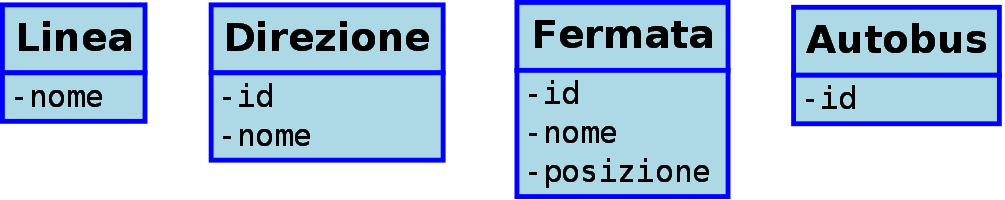
\includegraphics[width=12cm]{contents/images/classi_concettuali}
\end{center}
\caption{Classi concettuali}
\label{fig:classes}
\end{figure}

\newpage
Per ogni classe sono stati definiti anche i corrispettivi attributi d'interesse.

Nel caso della Linea, l'unico dettaglio di cui tenere traccia è il nome, che identifica univocamente la linea nell'insieme globale. Per quanto riguarda la direzione, essa è costituita da un nome di riferimento (usato solo per la consultazione) ed un ID, che ne permette la catalogazione.
Nel caso di Fermata, si può notare l'attributo nome, l'ID e la posizione ove la fermata è collocata, gestita attraverso una coordinata.
Per l'elemento Autobus, l'unico attributo di rilevanza è un ID, il quela permette di identificare un autobus in un vasto insieme di trasporti.

A questo punto si prosegue attraverso la concezione delle relazioni e la creazione delle associazioni tra classi.
Seguendo sempre il caso d'uso descritto in precedenza, una linea contiene un elenco di direzioni, mentre ogni direzione appartiene ad una e una sola linea. Viene quindi creata l'associazione ``Costituita da'' tra Linea e Direzione con molteplicità 1 a N.
Proseguendo, si può notare come a sua volta ogni direzione sia composta da un cospicuo numero di fermate, mentre una fermata può essere un punto di scambio tra più direzioni. Dunque l'associazione ``Composta da'' tra Direzione e Fermata avrà molteplicità N a N.
Concludendo con l'ultima classe, un autobus è associato ad'una direzione univoca e, durante il suo tragitto, si ferma in ogni fermata definita dalla direzione. In una direzione transitano più autobus e, allo stesso modo, in una fermata possono fermare più autobus. Le relazioni tra Autobus e Direzione e Autobus e Fermata saranno definite rispettivamente dall'associazione ``Appartiene'' di molteplicità N a 1 e dall'associazione `Collocato su'' di molteplicità N a 1.
\newpage
Avendo quindi specificato tutte le associazioni essenziali, il diagramma del modello di dominio assume questa forma:
\vspace{1cm}
\begin{figure}[htbp]
\begin{center}
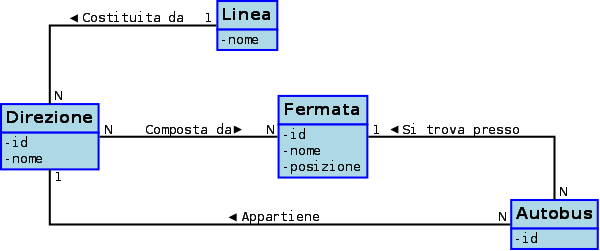
\includegraphics[width=12cm]{contents/images/modelloDominio}
\end{center}
\caption{Classi concettuali}
\label{fig:domain_model}
\end{figure}
\vspace{1cm}
La rappresentazione finale del modello di dominio di questo caso di studio è un diagramma molto semplice e snello, racchiudendo solamente i dettagli essenziali per la progettazione del servizio descritto in questo elaborato.
Come già spiegato in precedenza, il suo scopo non è descrivere in maniera esaustiva il comportamento di un servizio di trasporti urbani, ma si limita a definirne una concezione semplificata e, allo stesso tempo, sufficientemente completa per poter progettare un servizio efficiente.

Nel capitolo seguente si farà riferimento a questo modello di dominio per la definizione del {\itshape diagramma delle classi di progetto}, il quale si assumerà il compito di adattare la visione del modello ad un punto di vista software.
% section il_modello_della_rete_trasporti_pubblici (end)

\newpage